\section{Authoring Tools for XR}
\todo{THIS SECTION MUST BE EXTENDED WITH VR AUTHORING TOOLS BECAUSE IT HAS BEEN DONE ONLY FOR THE KTH PART}
\label{sec:background-authoring}

In the following section an exhaustive background of this thesis is provided for a better understanding of the research field and the related works in this topic. The chapter starts with \autoref{sec:ar-authoring} entering into details of the authoring tools and their categorization. Later, \autoref{sec:related-works} presents a literature review of authoring tools divided into programming tools (Subsection \autoref{subsec:related-programming-tools}) and content design tools (Subsection \autoref{subsec:related-content-design-tools}), with emphasis on the immersive ones (Subsection \autoref{subsec:related-immersice-hcdf}).

\subsection{AR Authoring}
\label{sec:ar-authoring}
The continuous growth of consumer electronics as smartphones and their computational power has led to an increasing interest in AR applications, thanks to their ability to engage the users.
However the process to create an AR application requires a long and time-consuming pipeline, involving expertise in different areas such as computer science and 2D/3D graphic design. The latter is especially needed when dealing with complex and accurate 3D models, which can be modeled with CAD tools (e.g. AutoCAD\footnote{https://www.autodesk.com/products/autocad/overview}, SolidWorks\footnote{https://www.solidworks.com}) and then converted using a DCC software (e.g. Blender\footnote{https://www.blender.org}) in a suitable file format for AR engines \cite{de_paolis_waat_2020}.

To facilitate and speed up the development of AR experiences several authoring tools have been proposed and commercialized: the authoring tools can be categorized into programming tools and content design tools \cite{marcus_authoring_2016}. While the former tools represent IDEs, frameworks or high-level APIs, the latter add various levels of abstractions reducing or, in some cases, removing the programming capability given their content driven nature.
In their work, Roberto et al. also provide a further classification of these tools depending on the level of application interface abstraction and concept abstraction, as seen in \autoref{fig:authoring-tools}.
\begin{figure}[]
	\centering
	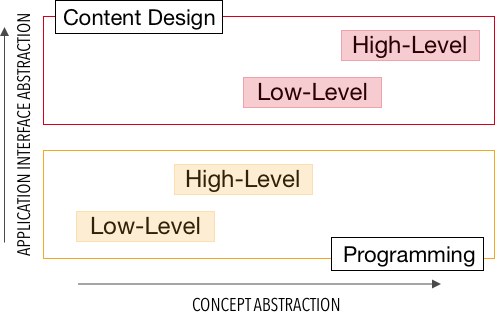
\includegraphics[width=8.5cm]{Background/authoring-tools.png}
	\caption{Categorization of AR authoring tools \cite{marcus_authoring_2016}.}
	\label{fig:authoring-tools}
\end{figure}
The two categories described above are organized into low-level and high-level. Programming tools are distinguished among those ones using low-level coding (i.e. requiring access to system primitives) and those working with high-level libraries.
Increasing the abstraction level of these tools we find the low-level content design tools, that require some scripting skills to add behaviors to AR contents; high-level content design tools, also known as High-Level Content Design Frameworks (HCDF), on the other hand abstract from the coding layer through a visual programming logic. This allows non-programmers to focus more on the interactions and behaviors of objects than their renderings.

Another classification of authoring tools is provided by Nebeling and Speicher \cite{nebeling_trouble_2018}, without a specific focus on AR experiences but instead considering both AR and VR applications. They based their classification on the level of fidelity achieved using a specific tool and the skills and resources required by the users to use it.

Apaza et al.~\cite{apaza_systematic_2018} focused their investigation in HCDFs through a systematic mapping and analysis of the current trends in the context of this development approach. 
They found that, after a first period dominated by the PC where the most common user interfaces were 2D and Non-immersive 3D, the development platform have been moving to different platforms as the web, HHD and HMD, with an increasing interest into immersive 3D user interfaces. The authors consider the authoring tools with an immersive 3D UI a “hot topic” given their WYSIWYG nature of editors.

\subsubsection{Development and Deployment Paradigms}
In \cite{marcus_authoring_2016} is described an analysis on the authoring and deployment paradigms of AR authoring tools. Two approaches characterize the authoring process: Stand-Alone and AR Plug-In.
The \textbf{Stand-Alone} approach is adopted by authoring solutions that include all the components required for a complete development of AR applications, as a GUI, rendering engines, and tracking options. The \textbf{AR Plug-In} paradigm uses, instead, a third-party component acting as plugin for a target software that, natively, would not support AR authoring. This components usually consist of GUI elements to configure a desired experience.

The last important step at the end of the authoring process is the deployment, consisting in two different strategies: the Platform-Specific and Platform-Independent methods. A \textbf{Platform-Specific} (PS) deployment builds the AR project in as many software packages as the number of deployment targets, being these native applications for a specific OS and, sometimes, hardware. 
The most interesting approach is, undoubtedly, the \textbf{Platform-Independent} (PI) deployment. It allows to export each AR experience in data files to be read on an AR browser acting as software platform (SP) running on the end-user device with the advantage that only one app is needed for multiple contents. A commercial example is given by Layar\footnote{https://layar.com}.\\
By combining the authoring and deployment paradigms presented above the authors based their research, describing four dataflow models belonging to AR content design tools.

\subsection{Related Work}
\label{sec:related-works}
Over the years, several authoring software and programming environments have emerged in the field of AR applications development. This section gives an understanding of these tools, divided by their abstraction level, with a particular focus on Content Design Tools and their sub-branch of Immersive Content Design Tools.
\subsubsection{Programming Tools}
\label{subsec:related-programming-tools}
AR authoring programming tools can consist of IDEs, libraries or frameworks and are usually used in combination with other tools to boost the authoring process.
These libraries are usually written in a low-level programming language like C/C++, therefore they require the user to have a specific programming knowledge. These libraries, of which ARToolkit\footnote{http://www.artoolkitx.org} \cite{kato1999marker} is one of the first examples, require the user to worry about low-level tasks such as marker tracking, spacial mapping or objects rendering \cite{stephanidis_authoring_2020},  while their high-level counterparts allow users to only code the interaction techniques or visualization of objects \cite{stephanidis_authoring_2020}.

Unity\footnote{https://unity.com} is an example of high-level programming tool, it is a professional game development environment that allows to visualize and manipulate simulations of AR scenes, moving geometries into them and editing their appearance. However, to author interactions, Unity requires coding through the C\# programming language and the AR functionalities are added by the Vuforia SDK\footnote{https://www.ptc.com/en/products/vuforia}, supporting features like tracking and visualization of contents.

\subsubsection{Content Design Tools}
\label{subsec:related-content-design-tools}
Content design tools require little to zero knowledge of programming in favor of a GUI that allows interactions and content authoring. Although very easy for rapid prototyping of AR applications, they may limit the customization of the designed experience achieved through programming tools.

DART (Designer's AR Toolkit), a plugin for Adobe Director now out of commerce, is an example of the earliest low-level content design tools. It was intended for multimedia designers to test AR designs and turn storyboards into minimum viable products by adding behaviors to objects either by dragging and dropping or by writing scripts using the Lingo scripting language. Wikitude Studio\footnote{https://www.wikitude.com/products/studio/} allows to create AR contents to be exported and read by the Wikitude AR browser app with a simple drag and drop interface of the editor and its workflow; Amazon Sumerian\footnote{https://aws.amazon.com/sumerian/}, instead, can be used to build quick AR web experiences accessible by mobile browsers on AR-enabled devices starting from .fbx 3D models to be added into the scene view.\\
HoloBuilder \cite{nebeling_trouble_2018} is a high-level tool defined by the authors as “a PowerPoint for AR applications”; it enables everyone to design experiences based on custom images or point clouds\footnote{https://en.wikipedia.org/wiki/Point\_cloud} as markers and the changes of states of the app is represented by the change of different “slides”. The authors also highlight several problems of HoloBuilder which are exploited to design a better tool, as the two proposed in their paper: ProtoAR and GestureWiz, both inspired by DART. Another similar tool is described in Villanueva et al.~\cite{villanueva_meta-ar-app_2020}, in which an authoring software for educators shows a canvas in which object animations can be created by choosing two points of the path that is automatically computed, while both QR code tracking and ground detection augmentation methods are supported.
SimpleAR has been defined as the HCDF aimed at users with no programming knowledge \cite{apaza-yllachura_simplear_2019} and it can be adapted to any AR programming framework given its framework abstraction. Indeed, end users can easily create mobile AR apps by calling primitive methods as obtaining a 3D model or triggering change of states after events by building the application logic through a visual programming editor in Google Blockly\footnote{https://developers.google.com/blockly/} as web app. A viewer, finally, shows the AR application modeled in the editor, reading the configuration from a Firebase database and downloading the 3D models through Google Poly\footnote{https://blog.google/products/google-ar-vr/poly-browse-discover-and-download-3d-objects-and-scenes/} APIs.
Another example of low-level content design tool is given by Lécuyer et al.~\cite{lecuyer_authoring_2019}, in which the proposed authoring tool exploits and adopts the object-relation paradigm already known in VR development, dividing the tool in a designer's part for the content authoring and a developer's part to implement the interactions. The created content is exported in a Unity project containing data about the scene, the interactions and tracking information, to allow a separation of concerns in favor of code re-usability.
Kurt et al.~\cite{kurt_argent_2020} analyze the processes involved in AR application development and, in their work, propose a pipeline of standardized processes called ARgent framework. The workflow steps consist of \textit{Uploading Assets}, \textit{Importing Assets}, \textit{Creating Animations}, \textit{Scripting} and \textit{AR-based Application testing}. The architecture of  this framework consists of a web interface written in HTML and JavaScript communicating with a WebServer connected to the database, this is used for assets management while scripting capabilities are achieved through the JavaScript programming language; eventually, the testing process allows the designer to experience the AR scene created, using methods as marker tracing or ground plane tracking.
A peculiar and interesting way to design AR experiences is proposed and implemented in the work by Shekhar et al.~\cite{shekhar_arcomposer_2019}: ARComposer, indeed, is a mobile application that leverages the advances in machine learning text analysis techniques to provide an interface where the authoring of AR scenes is entirely described by text; spacial arrangements are predicted as well as additional common objects are added based on common-world knowledge, and it supports both static and dynamic scenes.

\subsubsection{Immersive Content Design Tools}
\label{subsec:related-immersice-hcdf}
3D GUI authoring tools are examples of immersive authoring tools, proposed by Lee et al.~\cite{lee2005immersive}, in which objects' behaviors and interactions are defined within the same AR interface that shows them. They are usually deployed on HMD devices but in some cases HHDs are also a good alternative, allowing in-situ authoring of experiences and direct manipulation of 3D objects.

Yang et al.~\cite{yang_interactive_2016} provide one of the first examples, an AR development environment without programming, where contents are directly rendered by a HMD and user inputs are registered through a mobile device, that provides audio and haptic feedback. CAVE-AR \cite{cavallo_cave-ar_2019}, instead, uses VR to simulate the AR environment in which the experience is designed, independently of users' devices, blending the coordinate system of the two environments, mixing geographical information, architectural details and sensor data to debug the context of a typical AR use case scenario.

WAAT\footnote{Workstation AR Authoring Tool} \cite{de_paolis_waat_2020} is an AR authoring tool dedicated to training in industrial environments, in which line managers without a specific development knowledge can quickly create 3D scenes of workstations by placing 3D objects inside them. The system is composed of a desktop 3D authoring module, used to create the 3D scene, and an HMD module to place and manipulate 3D models in the augmented environment; the data tier is implemented by a server that exchanges a JSON file for each scene between the desktop and AR clients, while the hardware platform is the Microsoft Hololens 2\footnote{https://www.microsoft.com/en-us/hololens/hardware}. The desktop authoring task is performed with a mouse and a keyboard, through simple interactions as the drag and drop to place, move and change some properties of 3D objects; the HMD authoring task consists of a verification of the correct position, rotation and size of 3D models compared to the real objects, with the possibility to place or scale them via gestures to match the desired placement.
A comparison of this tool with Microsoft Dynamics 365 Guides\footnote{https://dynamics.microsoft.com/en-us/mixed-reality/guides/} shows a slightly faster authoring using the system of Béogut et al. given the already placed objects at the right position, resulting in a longer desktop authoring in favor of a shorter AR authoring task.\\
Also Story ARtist \cite{kegeleers_story_2021} uses JSON configuration files for an easy data management of assets and authored interactions in a prototype AR HMD application to create simple linear stories with Microsoft HoloLens.